\renewcommand{\relPath}{SECTION/20_Theory}
\chapter[Theory]{Theory of Optical Trapping}\label{ch:theory}

\lipsum[1-5]

\begin{figure}[htp]
  \centering
  % \tikzsetnextfilename{V_quadrant}
%%%%%%%
% READ TABLE
%%%%%%%
\pgfplotstableread{\relPath/10_Figures/TikZ/V_mat.dat}{\data}

\renewcommand{\tikzHelper}{
  \draw[black] (-1,0,0)--(1,0,0);
  \draw[black] (0,-1,0)--(0,1,0);
  \draw[black] (0,0,0) circle (1);
  }

\pgfplotsset{%
    colormap={bwr}{
      color=(blue);
      color=(white);
      color=(red);
    }%
}
%%%%%%%%%%%%%%%%%%%%%%%%%%%%%%%%%%
% Voltages per Quadrant
%%%%%%%%%%%%%%%%%%%%%%%%%%%%%%%%%%

\begin{tikzpicture}
  \begin{groupplot}[view={0}{90},
    % xlabel=$x$,
    % ylabel=$y$,
    height=5cm,
    width=5cm,
    point meta min=0,
    point meta max=1,
    colormap={}{ gray(0cm)=(1); gray(1cm)=(0);},
    group/xlabels at = edge bottom,
    group style = {
      group size = 2 by 2,
      horizontal sep=5mm,
      vertical sep=5mm,
      xlabels at = edge bottom,
      ylabels at = edge bottom
    }]

    \nextgroupplot[
      xticklabels={,,},
      ylabel={$\sfrac{y_{0}}{\RA}$},
    ]
        \addplot3[surf,mesh/rows=99,shader=interp] table[x=x,y=y,z=V4] {\data};
        \tikzHelper

    \nextgroupplot[
      yticklabels={,,},
      xticklabels={,,},
      colorbar right,
      every colorbar/.append style={
        ylabel={Normalized Voltage $\normalized{V}$},
        height=2*\pgfkeysvalueof{/pgfplots/parent axis height}+
        \pgfkeysvalueof{/pgfplots/group/vertical sep}}]
        \addplot3[surf,mesh/rows=99,shader=interp] table[x=x,y=y,z=V1] {\data};
        \tikzHelper

    \nextgroupplot[
      xlabel={$\sfrac{x_{0}}{\RA}$},
      ylabel={$\sfrac{y_{0}}{\RA}$},
    ]
        \addplot3[surf,mesh/rows=99,shader=interp] table[x=x,y=y,z=V3]
        {\data};
        \tikzHelper

    \nextgroupplot[
      xlabel={$\sfrac{x_{0}}{\RA}$},
      yticklabels={,,},
    ]
        \addplot3[surf,mesh/rows=99,shader=interp] table[x=x,y=y,z=V2] {\data};
        \tikzHelper


  \end{groupplot}
\end{tikzpicture}

  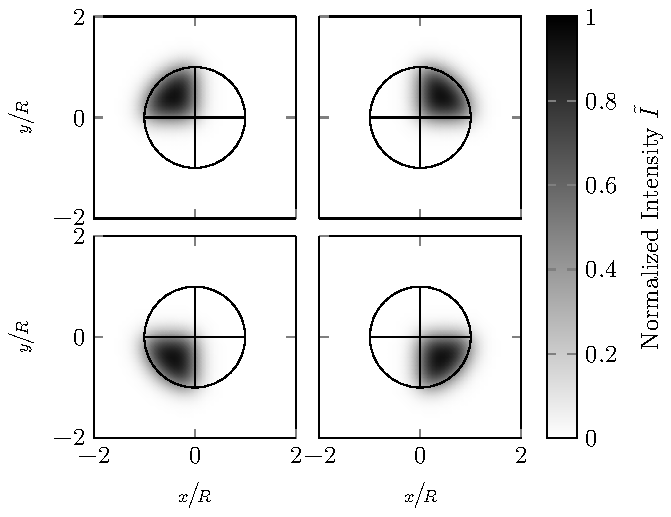
\includegraphics[]{Plots/cache/V_quadrant.pdf}
  \caption{Caption}
  \label{fig:Th-quadrant_Intensity}
\end{figure}

\lipsum[1-5]
\begin{figure}
  \centering
  \begin{subfigure}[b]{0.35\textwidth}
    \centering
    % \tikzsetnextfilename{QPDx}

\renewcommand{\tikzHelper}{
  \draw[black] (-1,0,0)--(1,0,0);
  \draw[black] (0,-1,0)--(0,1,0);
  \draw[black] (0,0,0) circle (1);

  \draw[black, dotted] (-1.5,0,0) -- (1.5,0,0);
  \draw[black, dotted] (-1.5,-0.6,0) -- (1.5,-0.6,0);
  \draw[black, dotted] (-1.5,0.6,0) -- (1.5,0.6,0);
}

\begin{tikzpicture}
  \begin{axis}[view={0}{90},
      xlabel=$\sfrac{x_{0}}{\RA}$,
      ylabel=$\sfrac{y_{0}}{\RA}$,
      point meta min=-1,
      point meta max=1,
      height=48mm,
      width=48mm,
      colormap/PuOr-11,
      colorbar,
      colorbar horizontal,
      colorbar style={
        title={\footnotesize Normalized Voltage $\normalized{V}_{x}$},
        at={(0,1.4)},
        anchor=north west,
        xtick={-1,0,1},
      }
    ]
      \addplot3[surf,mesh/rows=99,shader=interp] table[x=x,y=y,z=Vy] 
      {\relPath/10_Figures/TikZ/V_mat.dat};
    \tikzHelper
  \end{axis}
\end{tikzpicture}

    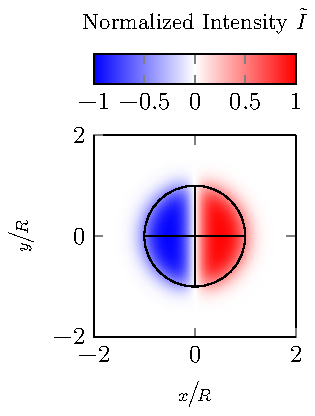
\includegraphics[]{Plots/cache/QPDx.pdf}
    \caption{Caption}
    \label{fig:Th-QPDx}
  \end{subfigure}
  \hfill
  \begin{subfigure}[b]{0.3\textwidth}
    \centering
    % \tikzsetnextfilename{QPDy}

\renewcommand{\tikzHelper}{
  \draw[black] (-1,0,0)--(1,0,0);
  \draw[black] (0,-1,0)--(0,1,0);
  \draw[black] (0,0,0) circle (1);
}

\pgfplotsset{%
    colormap={bwr}{
      color=(blue);
      color=(white);
      color=(red);
    }%
}

\begin{tikzpicture}
  \begin{axis}[view={0}{90},
      xlabel=$\sfrac{x}{\R}$,
      yticklabels={,,},
      point meta min=-1,
      point meta max=1,
      height=50mm,
      width=50mm,
      colorbar,
      colorbar horizontal,
      colorbar style={
        title={\footnotesize Normalized Intensity $\normalized{\intensity}$},
        at={(0,1.4)},
        anchor=north west,
        xtick={-1,-0.5,...,1},
      }
    ]
      \addplot3[surf,mesh/rows=51,shader=interp] table[x=x,y=y,z=Vx] 
      {\relPath/10_Figures/TikZ/V_mat.dat};
    \tikzHelper
  \end{axis}
\end{tikzpicture}

    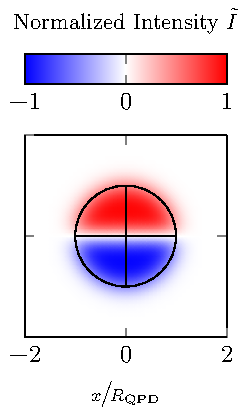
\includegraphics[]{Plots/cache/QPDy.pdf}
    \caption{Caption}
    \label{fig:Th-QPDy}
  \end{subfigure}
  \hfill
  \begin{subfigure}[b]{0.3\textwidth}
    \centering
    % \tikzsetnextfilename{QPDt}

\begin{tikzpicture}
  \begin{axis}[view={0}{90},
      xlabel=$\sfrac{x_{0}}{\RA}$,
      yticklabels={,,},
      height=48mm,
      width=48mm,
      colormap name=WhiteOr,
      colorbar,
      colorbar horizontal,
      colorbar style={
        title={\footnotesize Normalized Voltage $\normalized{V}_{t}$},
        at={(0,1.4)},
        anchor=north west,
        xtick={0,0.5,1},
      }
    ]
      \addplot3[surf,mesh/rows=99,shader=interp] table[x=x,y=y,z=V] 
      {\relPath/10_Figures/TikZ/V_mat.dat};

  \draw[black] (-1,0,0)--(1,0,0);
  \draw[black] (0,-1,0)--(0,1,0);
  \draw[black] (0,0,0) circle (1);

  \draw[black, dotted] (-1.5,0,0) -- (1.5,0,0);
  \draw[black, dotted] (-1.5,-0.6,0) -- (1.5,-0.6,0);
  \draw[black, dotted] (-1.5,0.6,0) -- (1.5,0.6,0);
  \end{axis}
\end{tikzpicture}

    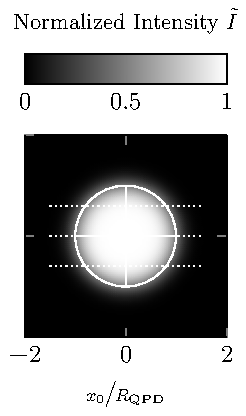
\includegraphics[]{Plots/cache/QPDt.pdf}
    \caption{Caption}
    \label{fig:Th-QPDt}
  \end{subfigure}
  \caption{QPDs}
  \label{fig:QPDs}
\end{figure}

\lipsum[1-5]

\begin{figure}[htp]
  \centering
  % \tikzsetnextfilename{Snell}

\tikzstyle arrowstyle=[scale=1]

\tikzstyle directed=[postaction={decorate,decoration={markings,
    mark=at position .65 with {\arrow[arrowstyle]{stealth}}}}]

\tikzstyle reverse directed=[postaction={decorate,decoration={markings,
    mark=at position .65 with {\arrowreversed[arrowstyle]{stealth};}}}]

\tikzset{SnellNode/.style={text width=10mm, align=center}}

\begin{tikzpicture}
  \def\W{5}
  \def\H{4}
  \def\x{0.95}
  \def\anglealpha{0}
  \pgfmathsetmacro{\y}{{(1-\x)*\H}}
  \pgfmathsetmacro{\radius}{(\W^2+\y^2)/2/\y}
  \pgfmathsetmacro{\anglealpha}{{asin(\W/\radius)}}
  \pgfmathsetmacro{\s}{{90+\anglealpha}}
  \pgfmathsetmacro{\e}{{90-\anglealpha}}

  \pgfmathsetmacro{\anglebeta}{{0.8*\anglealpha}}
  \pgfmathsetmacro{\p}{{(\radius-\H)*sin(\anglebeta)}}
  \pgfmathsetmacro{\px}{{\radius*sin(\anglebeta)}}
  \pgfmathsetmacro{\py}{{-\radius*(1-cos(\anglebeta))}}


  % define coordinates
  \coordinate (O) at (0,0) ;
  \coordinate (A) at (0,\H) ;
  \coordinate (B) at (0,-\H) ;

  % media
  \fill[blue!20,opacity=.3] (-\W,0) rectangle (\W,\H);
  \fill[black!10!,opacity=.3] (-\W,0) rectangle (\W,-\H);
  \node[right, SnellNode] at (2,1.5) {{Fluid\\ $\nf$}};
  \node[left, SnellNode] at (-2,-2) {{Particle\\ $\ns$}};

  % axis
  \draw[dash pattern=on5pt off3pt] (A) -- (B) ;
  % normal
  \draw[|->, thick] (0,0) -- node[right, pos=1] {$\normalvector$} (0, 2.5);


  % ray representation
  \def\gamma{130}
  \draw[red, variable=\x, domain=2.5:\W, samples=100] (0,\H) plot 
  ({\x*cos(\gamma)-cos(\x*pi r*3)/4*sin(\gamma)},{sin(\gamma)*\x+cos(\x*pi 
  r*3)/4*cos(\gamma)});

  % rays
  \draw[red,ultra thick,reverse directed] (O) -- node[left, xshift=-1mm, 
  pos=0.2] {$P_{\mathrm{i}}$} (130:5.2);

  \draw[red,ultra thick,directed] (O) -- node[right, xshift=1mm, pos=0.2] 
  {$P_{\mathrm{r}}$} (50:5.2);

  \draw[blue,directed,ultra thick] (O) -- node[right, xshift=1mm, pos=0.2] 
  {$P_{\mathrm{t}}$} (-70:4.24);

  % particle circumference
  \draw (-\W,-\y) arc (\s:\e:\radius);
  \draw[black,->|,>=stealth'] (\p,-\H) -- node[right, pos=0.7] {$\R$} (\px, 
  \py);

  % angles
  \draw[->,>=stealth'] (0,1) arc (90:130:1);
  \draw[->,>=stealth'] (0,1) arc (90:50:1);
  \draw[->,>=stealth'] (0,-1.4) arc (270:290:1.4);

  \node[] at (280:1.8)  {$\transmitted$};
  \node[] at (110:1.4)  {$\incident$};
  \node[] at (70:1.4)  {$\refracted$};

\end{tikzpicture}

  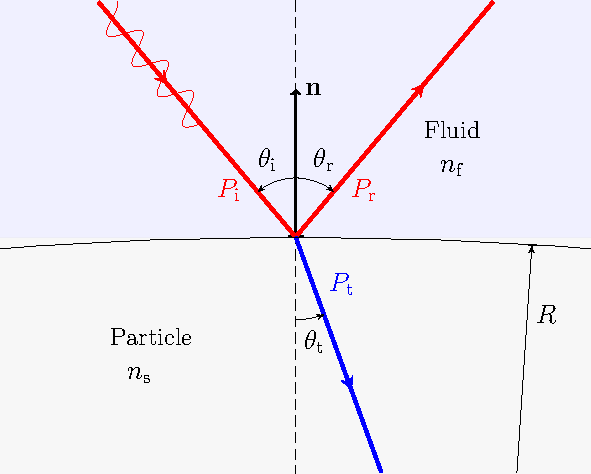
\includegraphics[]{Plots/cache/Snell.pdf}
  \caption{Caption}
  \label{fig:Th-snell}
\end{figure}

\lipsum[1-5]

\begin{figure}
  \centering
  \begin{subfigure}[b]{0.45\textwidth}
    \centering
    % \tikzsetnextfilename{gamma}
%%%%%%%
% READ TABLE
%%%%%%%

\begin{tikzpicture}
    \begin{axis}[view={0}{90},
        xlabel={$a$ [-]},
        ylabel={$\beta$ [\si{\degree}]},
        xmax=0.5,
        height=60mm,
        point meta min=0,
        point meta max=72,
        width=60mm,
        colormap/YlGnBu-9,
        colorbar,
        colorbar horizontal,
        colorbar style={
          title={$\gamma$ [\si{\degree}]},
          at={(0,1.3)},
          anchor=north west,
          xtick={0,24,48,72},
        },
        ytick={0,24,48,72},
        xtick={0,0.25,0.5},
      ]
      % countourf
      \addplot3[surf,mesh/rows=51,shader=interp] table[x=a,y=beta,z=gamma] 
      {\relPath/10_Figures/TikZ/angles_mat.dat};
      % lines
       \addplot3[
         mesh/rows=51,
         mesh/cols=50,
         contour gnuplot={levels={9,18,36,54},draw color=black},
     ] table[x=a,y=beta,z=gamma] {\relPath/10_Figures/TikZ/angles_mat.dat};

    \end{axis}
\end{tikzpicture}

    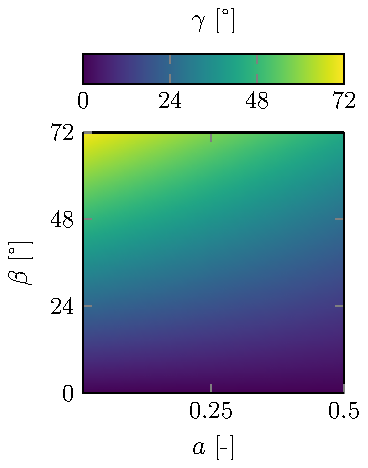
\includegraphics[]{Plots/cache/gamma.pdf}
    \caption{Caption}
    \label{fig:Th-gamma}
  \end{subfigure}
  \hfill
  \begin{subfigure}[b]{0.45\textwidth}
    \centering
    % \tikzsetnextfilename{theta_i}
%%%%%%%
% READ TABLE
%%%%%%%

\begin{tikzpicture}
    \begin{axis}[view={0}{90},
        xlabel={$a$ [-]},
        ylabel={$\beta$ [\si{\degree}]},
        xmax=0.5,
        height=60mm,
        point meta min=0,
        point meta max=30,
        width=60mm,
        colormap name=viridis,
        colorbar,
        colorbar horizontal,
        colorbar style={
          title={$\incident$ [\si{\degree}]},
          at={(0,1.3)},
          anchor=north west,
          xtick={0,10,20,30},
        },
        ytick={0,24,48,72},
        xtick={0,0.25,0.5},
      ]
      \addplot3[surf,mesh/rows=51,shader=interp] table[x=a,y=beta,z=theta] 
      {\relPath/10_Figures/TikZ/angles_mat.dat};
    \end{axis}
\end{tikzpicture}

    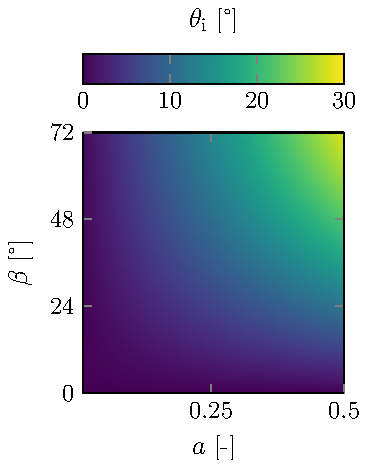
\includegraphics[]{Plots/cache/theta_i.pdf}
    \caption{Caption}
    \label{fig:Th-theta_i}
  \end{subfigure}
  \caption{angles}
  \label{fig:Th-gamma_theta}
\end{figure}

\lipsum[1-5]

\begin{figure}[htp]
  \centering
  % \tikzsetnextfilename{voltages_over_x}
%%%%%%%
% READ TABLE
%%%%%%%
\pgfplotstableread{\relPath/10_Figures/TikZ/V_line.dat}{\data}

\renewcommand{\tikzHelper}{
  \filldraw[black!10!, opacity=0.5] (-1,-1.1) rectangle (1,1.1);
}

\begin{tikzpicture}
\begin{groupplot}[
    group style={
        group name=myplot,
        group size= 1 by 3,
        vertical sep=8mm,
        },
    height=40mm,
    width=120mm,
    ymin=-1.1,
    ymax=1.1,
    ]
    \nextgroupplot[
    % ylabel={$\tilde{I}$},
      xticklabels={,,},
      title={$y = \sfrac{-0.64}{\RA}$},
      title style={yshift=-2mm},
      ]
      \tikzHelper
      \addplot[dotted] table[x=x,y=Vx_1] {\data};
      \addlegendentry{$V_{\MR{x}}$};
      \addplot[] table[x=x,y=Vy_1] {\data};
      \addlegendentry{$V_{\MR{y}}$};
      \addplot[dashed] table[x=x,y=V_1] {\data};
      \addlegendentry{$V_{\MR{t}}$};
    \nextgroupplot[
      % ylabel={$\tilde{I}$},
      title={$y = \sfrac{0}{\RA}$},
      title style={yshift=-2mm},
      xticklabels={,,},
      ylabel={Normalized Intensity $\normalized{\intensity}$},
      every axis y label/.append style={at=(ticklabel cs:0.5)}
      ]
      \tikzHelper
      \addplot[dotted] table[x=x,y=Vx_2] {\data};
      \addplot[] table[x=x,y=Vy_2] {\data};
      \addplot[dashed] table[x=x,y=V_2] {\data};
    \nextgroupplot[
      % ylabel={$\tilde{I}$},
      xlabel={$\sfrac{x}{\RA}$},
      title={$y = \sfrac{0.64}{\RA}$},
      title style={yshift=-2mm},
      ]
      \tikzHelper
      \addplot[dotted] table[x=x,y=Vx_3] {\data};
      \addplot[] table[x=x,y=Vy_3] {\data};
      \addplot[dashed] table[x=x,y=V_3] {\data};
\end{groupplot}
\end{tikzpicture}

  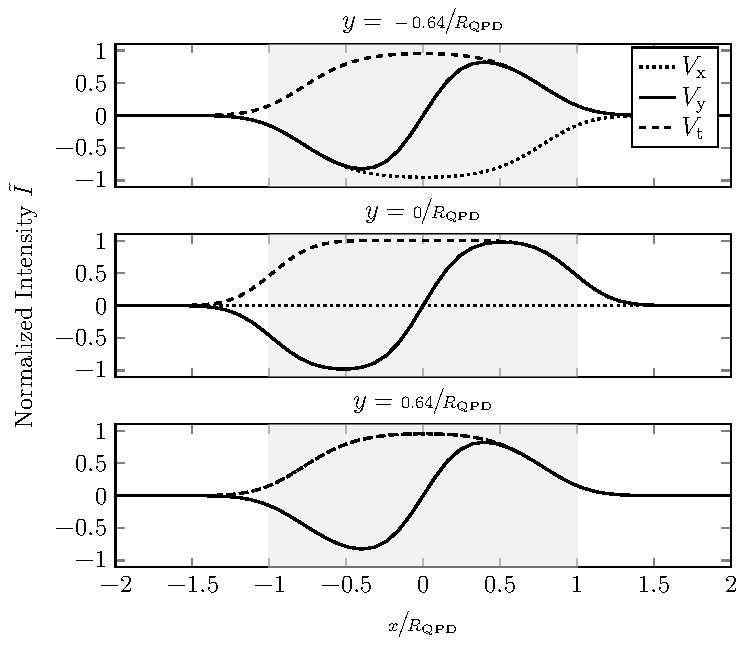
\includegraphics[]{Plots/cache/voltages_over_x.pdf}
  \caption{Fresnel}
  \label{fig:Th-voltages_over_x}
\end{figure}

\lipsum[1-5]

\begin{figure}[htp]
  \centering
  % \tikzsetnextfilename{Fresnel}
%%%%%%%
% READ TABLE
%%%%%%%
\pgfplotstableread{\relPath/10_Figures/TikZ/Fresnel.dat}{\data}

\begin{tikzpicture}
  \begin{groupplot}[
    axis on top=true,
    group style={
      group size=2 by 1,
      horizontal sep = 23mm,
    },
    xmin=0,
    ymin=0,
    height=55mm,
    width=73mm,
    no markers,
  ]
  \nextgroupplot[
    xlabel={Incident angle $\incident$ [\si{\degree}]},
    ylabel={\footnotesize Fresnel Coefficient [-]},
    xtick={0,0.16666,0.333333,0.5},
    xticklabels={0, 30, 60, 90},
    legend style={
      at={(axis cs:0.01,0.5)},
      anchor=west,
      font=\footnotesize,
    }
  ]
  \filldraw[black!10!,opacity=0.7] (0.155,0) rectangle ({0.5,1}|-{rel axis 
  cs:1,1});

    \addplot[dashed] table[x=theta,y=R_M2P] {\data};
    \addlegendentry{$\fresnelR_{\mathrm{f\rightarrow s}}$};
    \addplot[] table[x=theta,y=T_M2P] {\data};
    \addlegendentry{$\fresnelT_{\mathrm{f\rightarrow s}}$};

    \addplot[thick, blue, dotted] table[x=theta,y=R_P2M] {\data};
    \addlegendentry{$\fresnelR_{\mathrm{s\rightarrow f}}$};
    \addplot[thick, blue] table[x=theta,y=T_P2M] {\data};
    \addlegendentry{$\fresnelT_{\mathrm{s\rightarrow f}}$};

    \nextgroupplot[
    xlabel={Incident angle $\incident$ [\si{\degree}]},
    xmax=0.167,
    ymin=0.001,
    ymode=log,
    xtick={0,0.05555,0.11111,0.1666666},
    xticklabels={0, 10, 20, 30},
  ]

  \filldraw[black!10!,opacity=0.7] (0.155,0.00001) rectangle ({0.167,1}|-{rel 
  axis cs:1,1});

    \addplot[dashed] table[x=theta,y=R_M2P] {\data};
    \addplot[] table[x=theta,y=T_M2P] {\data};

    \addplot[thick, blue, dotted] table[x=theta,y=R_P2M] {\data};
    \addplot[thick, blue] table[x=theta,y=T_P2M] {\data};

  \end{groupplot}
  % \draw[thick,blue,->,shorten >=2pt,shorten <=2pt] (group c1r1.east) -- (group 
  % c2r1.west);
\end{tikzpicture}

  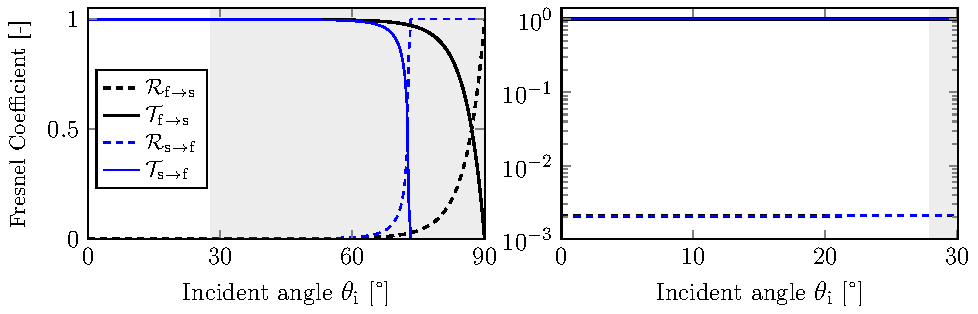
\includegraphics[]{Plots/cache/Fresnel.pdf}
  \caption{Fresnel}
  \label{fig:Th-fresnel}
\end{figure}

\lipsum[1-5]

\begin{figure}[htp]
  \centering
  % \tikzsetnextfilename{angles}

\tikzstyle arrowstyle=[scale=2]
\tikzstyle directed=[postaction={decorate,decoration={markings,
    mark=at position .65 with {\arrow[arrowstyle]{stealth}}}}]

\begin{tikzpicture}[scale=1.3]
    \coordinate (O) at (0,0);
    \coordinate (I) at (4,3);
    \coordinate (A) at (0,1.4);

    \node[circle,fill=black,inner sep=0pt,minimum size=3pt,label=below:{$M$}] 
    at (O) {};
    \node[circle,fill=black,inner sep=0pt,minimum size=3pt,label=left:{$f$}] at 
    (A) {};
    \node[circle,fill=black,inner sep=0pt,minimum size=3pt,label=above:{$I$}] 
    at (I) {};

    % \draw (O) -- node[midway, below, xshift=1mm] {$R$} (I) -- node[above, 
    % midway, xshift=-1mm] {$y$} (A) -- node[midway, left] {$a\,R$} cycle;
    \draw (O) -- node[midway, below, xshift=1mm] {$\R$} (I) -- (A) -- 
    node[midway, left] {$a\,\R$} cycle;

    % \draw[dotted] (O) rectangle (I);
    \draw[dotted] (A) -- ++(0,1);

    \draw[->,>=stealth'] (I) -- node[above,midway] {$\normalvector$} (36.86:6);

    \draw[directed,red] (34.0:6.2) -- (I);


    \draw[] (0,0.5) arc (90:37:0.5) node[midway, above] {$\gamma$};
    \draw[] (0,1.9) arc (90:22:0.5) node[midway, above] {$\beta$};
    \draw[] (0,1.1) arc (-90:22:0.3) node[midway, right] 
    {$\sfrac{\pi}{2}-\beta$};
    \draw[] (36.8:3.5) arc (216:200.5:1.5) node[pos=.3, left] {$\incident$};

    \draw[] (I) arc (36.86:48:5);
    \draw[] (I) arc (36.86:-3:5);

\end{tikzpicture}

  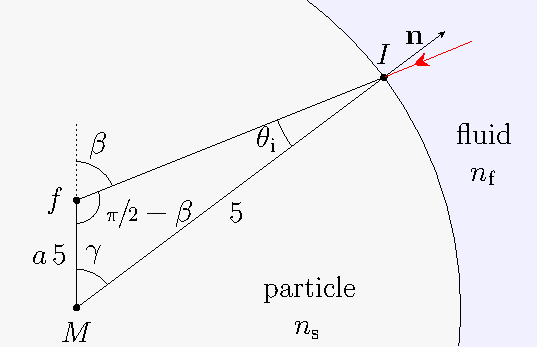
\includegraphics[]{Plots/cache/angles.pdf}
  \caption{Caption}
  \label{fig:Th-angles}
\end{figure}

\lipsum[1-5]

\begin{figure}[htp]
  \centering
  % \tikzsetnextfilename{ray}
{
\small

\tikzset{cross/.style={
  cross out,
  draw=black,
  minimum size=2*(#1-\pgflinewidth),
  inner sep=0pt, outer sep=0pt},
  cross/.default={1pt}}

\tikzstyle arrowstyle=[scale=2]

\tikzstyle directed=[postaction={decorate,decoration={markings,
    mark=at position .5 with {\arrow[arrowstyle]{stealth}}}}]

\tikzstyle reverse directed=[postaction={decorate,decoration={markings,
    mark=at position .65 with {\arrowreversed[arrowstyle]{stealth};}}}]

\begin{tikzpicture}[scale=1.5]

  % define coordinates
  \coordinate (O) at (0,0) ;
  \coordinate (F) at (0,0.15) ;
  \coordinate (N) at (260:2) ;

  % medium
  \filldraw[blue!20!, opacity=0.3] (-3,-3) rectangle ++(6,6);


  % particle
  \draw[fill=white] (O) circle (2);
  \draw[fill=black!10!, opacity=0.3] (O) circle (2);

  \node[circle, fill=black, inner sep=0pt, minimum size=3pt, label=left:{$M$}] 
  at (O) {};
  \node[circle, fill=black, inner sep=0pt, minimum size=3pt, label=above:{$f$}] 
  at (F) {};

  % rays
  \coordinate (I) at (28.6:2) ;
  \node[circle,fill=black,inner sep=0pt,minimum size=3pt,label=above:{$I$}] at 
  (I) {};
  \node[circle,fill=black,inner sep=0pt,minimum size=3pt,label=right:{$N$}] at 
  (N) {};
  \draw[directed,red] (2.5,1.3) -- node[below, midway] {$\power{i}{1}$} (I);
  \draw[directed,red] (N) -- node[left,xshift=-0.1mm] {$\power{t}{2}$} 
  (258:2.8);

  \draw[directed, blue] (I) -- node[right,midway,xshift=0.1mm] 
  {$\power{t}{1}=\power{i}{2}$} (N);

  \draw[directed, blue] (N) -- node[left,midway,xshift=-0.1mm] 
  {$\power{r}{2}=\power{i}{3}$} (131.4:2);

  % arcs
  \draw[<-,>=stealth'] ([shift=(234:0.5)]I) arc (234:209:0.5);

  \draw[<->,>=stealth'] ([shift=(55:0.5)]N) arc (55:105:0.5);

  \node[] at (22:1.2) {$\transmitted^{1}$};
  \node[] at (269:1.2) {$\incident^{2}$};
  \node[] at (254:1.22) {$\reflected^{2}$};

  % middle to hitting point
  \draw[densely dotted] (O) -- node[below,pos=0.3] {$\R$} (I);
  \draw[densely dotted] (O) -- node[left,pos=0.3] {$\R$} (N);
  \draw[red, dotted] (I) -- (F);
  % surface normal
  \draw[|->,>=stealth'] (N) -- node[right,pos=0.9] {$\normalvector$} (260:3);
  \draw[|->,>=stealth'] (I) --node[above,pos=0.9] {$\normalvector$} (28.6:3);

  % text
  \node[align=center, text width=15mm] at (-0.5,1) {{particle\\ $\ns$}};
  \node[align=center, text width=15mm] at (1.5,2) {{fluid\\ $\nf$}};

\end{tikzpicture}
}

  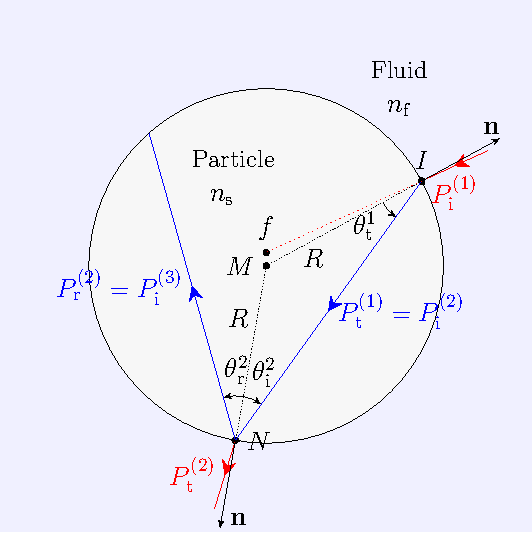
\includegraphics[]{Plots/cache/ray.pdf}
  \caption{Caption}
  \label{fig:Th-ray_particle}
\end{figure}
